\chapter {Background Study}
\label{background_study}
Base of a good research is the understanding of the background terms and definition. To understand the image processing and character reorganisation, one have to clearly understand about image filtering, image transformations and tesseract OCR Engine operation. In this chapter as background knowledge discovery we will discuss about some image processing term and tesseract.

\section{Gray Scale}
In photography and computing, a grayscale or greyscale digital image is an image in which the value of each pixel is a single sample, that is, it carries only intensity information. Images of this sort, also known as black-and-white, are composed exclusively of shades of gray, varying from black at the weakest intensity to white at the strongest. \cite{GrayScale}

\section{Blur}
Blurring is a very powerful operation used in image processing and procedural texture generation. Blurs involve calculating weighted averages of areas of pixels in a source image for each pixel of the final blurred image. Blurring images so they become fuzzy may not seem like a useful operation, but actually is very useful for generating background effects and shadows\cite{GaussianSmoothing}. In our form image blur operation increase border edges.

\subsection{Gaussian smoothing}
The Gaussian smoothing operator is a 2-D convolution operator that is used to `blur' images and remove detail and noise. The idea of Gaussian smoothing is to use this 2-D distribution as a `point-spread' function, and this is achieved by convolution. Since the image is stored as a collection of discrete pixels we need to produce a discrete approximation to the Gaussian function before we can perform the convolution. I Gaussian smoothing technique is widely used effect in graphics software, typically to reduce image noise and reduce detail. \cite{GaussianSmoothing}
\begin{figure}[H]
\centering
\label{fig:Blur} 
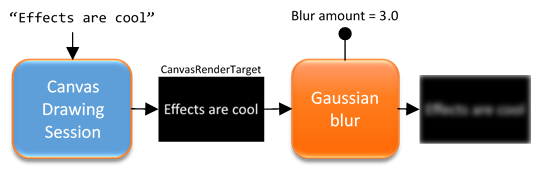
\includegraphics[width=0.8\textwidth]{Blur.png}
\caption {Gaussian smoothing}
\end{figure}

\section{Thresholding}
Thresholding is one of the most basic techniques for what is called Image Segmentation. When the threshold technique is applied on an image, we get segments inside the image and each of segments are represent something.\cite{Thresholding}
\begin{itemize}
\item Thresholding is a simple way of segmentation.
\item We separate out various regions of an image regarding to objects which we want to analyze. The object pixels and the background pixels are the backbone of this separation.
\item To differentiate the pixels we are interested in from the rest, we perform a comparison of each pixel intensity value with respect to a threshold.
\item Once we have separated properly the important pixels, we can set them with a determined value to identify.
\end{itemize}

\begin{figure}[H]
\centering
\label{fig:Thresholding} 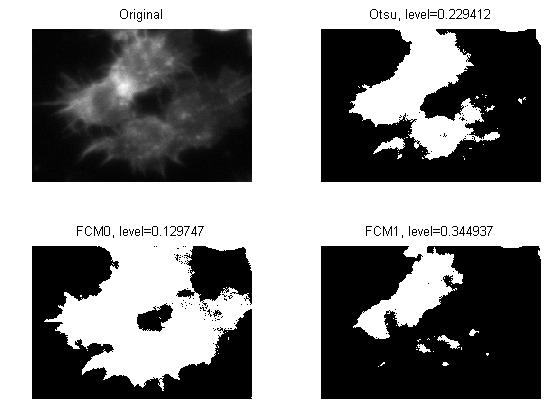
\includegraphics[width=0.8\textwidth]{Thresholding}
\caption {Thresholding}
\end{figure}


\section{Edge Detection}
In digital image processing, edge detection is an important subject matter. Edge detection is a crucial step in object recognition. It is a process of finding sharp discontinuities in an image. The discontinuities are abrupt changes in pixel intensity which characterize boundaries of objects in a scene. In short, the goal of edge detection is to produce a line drawing of the input image. \cite{EdgeDetection}

The Canny operator is also known as the optimal detector, developed by John F. Canny in 1986.  There are multiple steps to implement the Canny operator. First, a Gaussian filters is used to smooth the image to remove noise in an image. Second, compute the gradient magnitude. Third, apply the algorithm to remove the pixels that are not part of an edge. Last step is involved with the use of hysteresis thresholding along edges. Hysteresis is based on two thresholds which are upper and lower. If a pixel gradient is higher than the upper threshold, then the pixel will be marked as an edge and if a pixel gradient is below the lower threshold, then the pixel will be marked as a non-edge. \cite{CannyEdgeDetection}

\begin{figure}[H]
\centering
\subfloat [Original Image of a building]{\label{fig:EdgeOriginal1} 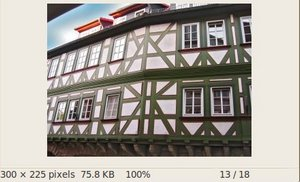
\includegraphics[width=0.6\textwidth]{EdgeOriginal}}
\subfloat [Edge Detected Image]{\label{fig:EdgeDetection1} 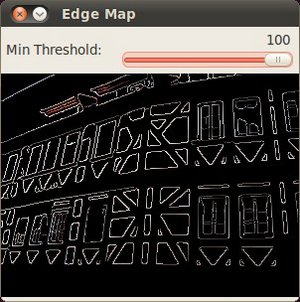
\includegraphics[width=0.5\textwidth]{EdgeDetect}}
\caption {Edge Detection}
\label {fig:EdgeDetection}
\end{figure}

\section{Contour}
Although algorithms like the Canny edge detector can be used to find the edge pixels that separate different segments. The next step is to be able to assemble those edge pixels into contours.
A contour is a list of points that represent, in one way or another, a curve in an image. This representation can be different depending on the circumstance at hand. There are many ways to represent a curve. Contours are represented in OpenCV by sequences in which every entry in the sequence encodes information about the location of the next point on the curve.

\begin{figure}[H]
\centering
\subfloat [Original Image]{\label{fig:ContourOriginal} 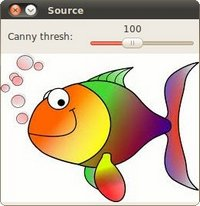
\includegraphics[width=0.4\textwidth]{ContureOriginal}}
\subfloat [Contour Detect]{\label{fig:Contour1} 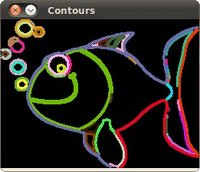
\includegraphics[width=0.4\textwidth]{Conture}}
\caption {Find Contour}
\label {fig:ContourDetection}
\end{figure}

\section{Tesseract OCR engine}
Tesseract is an open source optical character recognition (OCR) engine. HP was originally started it as a project. Later it was modified, improved and taken over by Google and later released as open source in year 2005\cite{TesseractORCEngine} \cite{TesseractORCEngineOfficialWeb}.

Tesseract is considered as one of the most accurate free software OCR engines currently available. A large variety of other OCR software now uses it as a base. It is an excellent quality OCR program, with a large amount of flexibility, a solid codebase, and a large, engaged community of interested people around it.

This thesis investigates the principles of optical character recognition used in the Tesseract OCR engine and techniques to improve its efficiency and runtime. 

Optical character recognition (OCR) method has been used in converting printed text into editable text in various applications over a variety of devices such as Scanners, computers, tablets etc. But now Mobile is taking over the computer in all the domains but OCR still remains one not so conquered field. This paper focuses on improving the Tesseract OCR efficiency for Bangla. 

This thesis presents a preprocessing technique being applied to the Tesseract Engine to improve the recognition of the characters keeping the runtime low.

\section{Why Tesseract}
The first relevant criterion in Tesseract is the fact that is free and open source (FOSS), which is an advantage and a key point in the research development.

Usually, whenever Tesseract is compared to another free OCR tool, it is the best whether in terms of recognition rate or speed. Even, when it is compared with the Finereader commercial tool, Tesseract arrives to rub it and managed to overtake for handwritten writing.

\section{Optical character recognition systems}
An OCR system is a system that takes a text image as input and applies certain treatments through modules making up the system in order to output editable file with the same text.

The architecture of an OCR system varies from one system to another as needed.Optical Character Recognition systems are usually composed of the following phases:

\begin{itemize}
\item Preprocessing phase: prepares the sensor data to the next phase. It is a set of treatments allowing image quality increasing.
\item Segmentation phase: delimits document elements (line, word, character ). By applying good segmentation techniques, we can increase the performance of OCR systems.
\item Feature extraction phase: defines features characterizing the delimited elements of a document. Feature extraction is one of the most important steps in developing a classification system. This step describes the various features characterizing the delimited elements of a document.
\item Classification phase: recognizes and identifies each element. It is performed based on the extracted features.
\item Post-processing phase: it is an optional phase. It may be automatic or manual.
\end{itemize}
Several approaches and techniques have been developed for each module.